%%%%%%%%%%%%%%%%%%%%%%%%%%%%%%%%%%%%%%%%%%%%%%%%%%%%%%%%%%%%%%%%%%%%%%%%%%%%%%
%%%%%%%%%%%%%%%%%%%%%%%%%%%%%%%%%%%%%%%%%%%%%%%%%%%%%%%%%%%%%%%%%%%%%%%%%%%%%%
%%
%% Dokumentace k projektu pro předmět ITU, 2013
%% Jednoduchý správce oken
%%
%%%%%%%%%%%%%%%%%%%%%%%%%%%%%%%%%%%%%%%%%%%%%%%%%%%%%%%%%%%%%%%%%%%%%%%%%%%%%%
%%%%%%%%%%%%%%%%%%%%%%%%%%%%%%%%%%%%%%%%%%%%%%%%%%%%%%%%%%%%%%%%%%%%%%%%%%%%%%
\documentclass[12pt,a4paper,titlepage,final]{article}

% matika
\usepackage[tbtags]{amsmath}
% cestina a fonty
\usepackage[czech]{babel}
\usepackage[utf8]{inputenc}
\usepackage[IL2]{fontenc}	% aby se text dal z PDF lehce kopírovat s diakritikou
% balicky pro odkazy
\usepackage[bookmarksopen,colorlinks,plainpages=false,urlcolor=blue,unicode]{hyperref}
\usepackage{url}
% obrazky
\usepackage[dvipdf]{graphicx}
\usepackage{float}
% velikost stranky
\usepackage[top=3.5cm, left=2.5cm, text={17cm, 24cm}, ignorefoot]{geometry}
% \usepackage{lscape}

\begin{document}

%%%%%%%%%%%%%%%%%%%%%%%%%%%%%%%%%%%%%%%%%%%%%%%%%%%%%%%%%%%%%%%%%%%%%%%%%%%%%%
% titulní strana

\begin{titlepage}

% \vspace*{1cm}
\begin{figure}[!h]
  \centering
  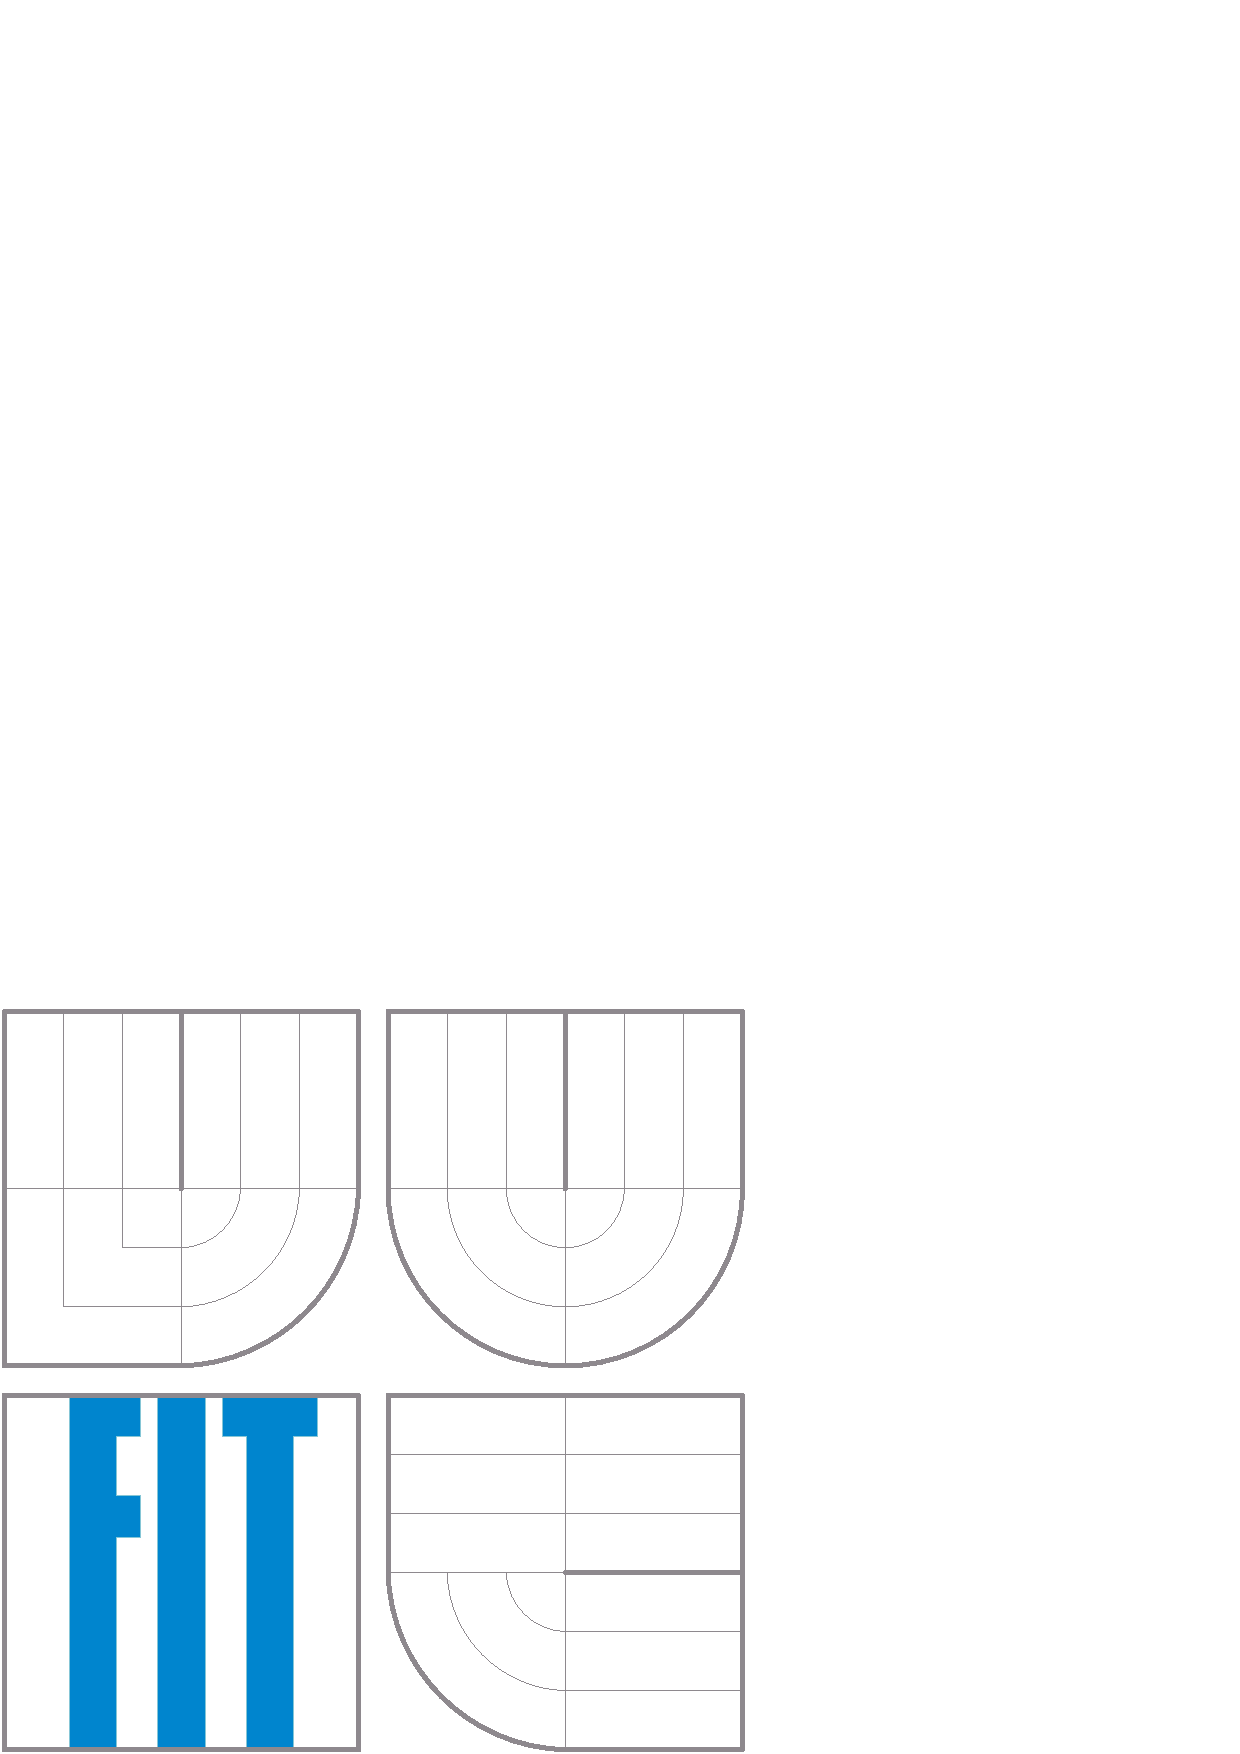
\includegraphics[height=5cm]{img/logo.pdf} \\
  Fakulta Informačních Technologií \\
  Vysoké Učení Technické v~Brně
\end{figure}

\vfill

\begin{center}
\begin{Large}
Dokumentace k projektu pro předmět ITU\\
\end{Large}
\bigskip
\begin{Huge}
Jednoduchý správce oken\\
\end{Huge}
\end{center}

\vfill

\begin{center}
\begin{Large}
\today
\end{Large}
\end{center}

\vfill

\begin{flushleft}
\begin{large}
\begin{tabular}{lll}
% * @author Biberle Zdeněk <xbiber00@stud.fit.vutbr.cz>
% * @author Doležal Jan    <xdolez52@stud.fit.vutbr.cz>
% * @author Kalina Jan     <xkalin03@stud.fit.vutbr.cz>
Autoři: & Zdeněk Biberle, & \href{mailto:xbiber00@stud.fit.vutbr.cz}{\nolinkurl{xbiber00@stud.fit.vutbr.cz}} \\
        & Jan Doležal,    & \href{mailto:xdolez52@stud.fit.vutbr.cz}{\nolinkurl{xdolez52@stud.fit.vutbr.cz}} \\
        & Jan Kalina,     & \href{mailto:xkalin03@stud.fit.vutbr.cz}{\nolinkurl{xkalin03@stud.fit.vutbr.cz}} \\
\end{tabular}
\end{large}
\end{flushleft}
\end{titlepage}


%%%%%%%%%%%%%%%%%%%%%%%%%%%%%%%%%%%%%%%%%%%%%%%%%%%%%%%%%%%%%%%%%%%%%%%%%%%%%%
% obsah
\pagestyle{plain}
\pagenumbering{roman}
\setcounter{page}{1}
%\tableofcontents

%%%%%%%%%%%%%%%%%%%%%%%%%%%%%%%%%%%%%%%%%%%%%%%%%%%%%%%%%%%%%%%%%%%%%%%%%%%%%%
% textova zprava
\newpage
\pagestyle{plain}
\pagenumbering{arabic}
\setcounter{page}{1}

% Do dokumentace (na rozdíl od prezentace) uveďte vše, co se týká vypracování projektu, jeho implementace a testování. Dokumentujte informační zdroje, ze kterých bylo čerpáno při řešení, vlastní myšlenky a přínos. Nepopisujte všeobecně známé věci a triviality. Podrobně vyjmenujte použité knihovny ve Vašem řešení a postup při jejich kompilaci s Vaší implementací. 

%%%%%%%%%%%%%%%%%%%%%%%%%%%%%%%%%%%%%%%%%%%%%%%%%%%%%%%%%%%%%%%%%%%%%%%%%%%%%%
\section{Úvod} \label{uvod}
%%%%%%%%%%%%%%%%%%%%%%%%%%%%%%%%%%%%%%%%%%%%%%%%%%%%%%%%%%%%%%%%%%%%%%%%%%%%%%

V této práci je řešena implementace a testování inovativního správce oken ``gawm''.
Jedná se o kompozitní správce oken pro grafické prostředí X, který umožňuje pracovat s okny v nekonečně velkém prostoru, po kterém se uživatel může pohybovat ve stylu CADových systémů a strategických her.

Cílem je přinést inovativní způsob práce s okny, umožňující pracovat s velkým množstvím oken bez potřeby abstraktní představy minimalizace nebo virtuálních ploch.

Jako každý správce oken umožňuje okna přesouvat, jejich minimalizaci se ale snaží nahradit konceptem virtuálních ploch, který je ale zbaven striktního rozdělení prostoru oken na jednotlivé virtuální plochy - okna leží na nekonečné ploše, jejíž výřez se uživateli zobrazuje a v kterém se může volně pohybovat a zoomovat pro dosažení maximální orientace v oknech.

Přebourává tak koncept virtuálních ploch podobným způsobem jakým aplikace 280slides.com přebourává koncept slidů prezentace.
Uživatel se po ploše pohybuje ve stylu CAD systémů, tažením myší po volné ploše, nebo ve stylu Real time strategy, umístěním kurzoru myši na hranu obrazovky.

Přidanou hodnotou aplikace může být možnost pracovat i se zmenšenými okny na odzoomované ploše.
Na rozdíl od náhledů aplikací známých například z Gnome Shell tak umožňuje s aplikacemi pracovat aniž by bylo nutné opustit režim náhledů (který je zde právě nahrazen prostým odzoomováním) a vyřešit tak i problémy s obtížným drag-and-drop mezi aplikacemi na různých virtuálních plochách.

%%%%%%%%%%%%%%%%%%%%%%%%%%%%%%%%%%%%%%%%%%%%%%%%%%%%%%%%%%%%%%%%%%%%%%%%%%%%%%
\section{Implementace}
%%%%%%%%%%%%%%%%%%%%%%%%%%%%%%%%%%%%%%%%%%%%%%%%%%%%%%%%%%%%%%%%%%%%%%%%%%%%%%

Projekt je implementován za pomocí knihovny Xlib \cite{Xlib} a OpenGL (nebyly požity žádné frameworky jako Clutter nebo Qt).
Jako verzovací systém byl použit systém GIT.
Na rozdíl od knihovny OpenGL bylo nutné knihovnu Xlib nastudovat, protože s ní nikdo neměl zkušenosti.

Na webu jsme našli vzor minimálního kompozitního správce oken \cite{min_comp_wm}, ze kterého jsem zjistili jak je složité napsat správce oken.
Použití kompozice bylo nutné pro implementaci zoomování.
Částečně z toho důvodu jsme také použili OpenGL, aby jsme měli podporu hardwarového vykreslování.

Postupně se ukázalo rozhraní systému Xwindow jako nedostatečné a to hlavně z důvodu odchytávání událostí a asynchronnosti.
Událost je nemožné odchytit a při tom odeslat aplikaci.
Mezitím co jsme vykreslovali okno, docházelo ke zmizení pixmapy.
Vykreslování tedy často končí odmítnutím spojení s Xserverem a následným pádem našeho správce oken.

%%%%%%%%%%%%%%%%%%%%%%%%%%%%%%%%%%%%%%%%%%%%%%%%%%%%%%%%%%%%%%%%%%%%%%%%%%%%%%
\section{Testování}
%%%%%%%%%%%%%%%%%%%%%%%%%%%%%%%%%%%%%%%%%%%%%%%%%%%%%%%%%%%%%%%%%%%%%%%%%%%%%%

Popsaný správce oken má za cíl přinést styl práce z průmyslem prověřených CADových aplikací a intuitivní principy osvědčené v herním průmyslu do prostředí správy oken.
Hlavní cílovou skupinou jsou tak lidé zvyklí pracovat s CADovými systémy a podobnými aplikacemi a (současní a bývalí) hráči strategických her.

Beta-testování na cílové skupině bohužel nebylo provedeno, neboť se nepodařilo produkt odladit natolik,
aby prošel alfa-testováním jeho vývojáři. Strojaři nicméně byly nadšení při náznaku možnosti příchodu správce
oken užívajících popsaných principů.

%%%%%%%%%%%%%%%%%%%%%%%%%%%%%%%%%%%%%%%%%%%%%%%%%%%%%%%%%%%%%%%%%%%%%%%%%%%%%%
\section{Závěr} \label{zaver}
%%%%%%%%%%%%%%%%%%%%%%%%%%%%%%%%%%%%%%%%%%%%%%%%%%%%%%%%%%%%%%%%%%%%%%%%%%%%%%

Je velká škoda že se správce oken nepodařilo dovést ke stabilní a implementaci, která by umožnila práci s okny
i po odzoomování/přizoomování. Bohužel okenní systém X neposkytuje jednoduchou cestu jak uvedené implementovat,
mnohem úspěšnější by mohla implementace být při použití okenního systému Wayland, který ale bohužel není v současné
době dostatečně stabilní a nebyl ani dostatek času na kompletní přepracování implementace od samého základu.

%%%%%%%%%%%%%%%%%%%%%%%%%%%%%%%%%%%%%%%%%%%%%%%%%%%%%%%%%%%%%%%%%%%%%%%%%%%%%%
% seznam citované literatury: každá položka je definována příkazem
% \bibitem{xyz}, kde xyz je identifikátor citace (v textu použij: \cite[poznámka]{xyz})
\begin{thebibliography}{1}

\bibitem{Xlib}
\href{http://tronche.com/gui/x/xlib/}{Xlib} \newline
\href{http://tronche.com/gui/x/xlib/}{\nolinkurl{http://tronche.com/gui/x/xlib/}}

\bibitem{min_comp_wm}
\href{http://wingolog.org/archives/2008/07/26/so-you-want-to-build-a-compositor}{Minimální kompozitní správce oken} \newline
\href{http://wingolog.org/archives/2008/07/26/so-you-want-to-build-a-compositor}{\nolinkurl{http://wingolog.org/archives/2008/07/26/so-you-want-to-build-a-compositor}}

\end{thebibliography}
%%%%%%%%%%%%%%%%%%%%%%%%%%%%%%%%%%%%%%%%%%%%%%%%%%%%%%%%%%%%%%%%%%%%%%%%%%%%%%
% přílohy
%\pagebreak
%\appendix

%%%%%%%%%%%%%%%%%%%%%%%%%%%%%%%%%%%%%%%%%%%%%%%%%%%%%%%%%%%%%%%%%%%%%%%%%%%%%%
%\section{Příloha: Něco}
%%%%%%%%%%%%%%%%%%%%%%%%%%%%%%%%%%%%%%%%%%%%%%%%%%%%%%%%%%%%%%%%%%%%%%%%%%%%%%

\end{document}
